\documentclass[oneside]{nccuthesis}

\usepackage{times}
\usepackage{verbatim}
\usepackage{color}
\usepackage{url}
\usepackage{graphicx}
\usepackage{array}
\usepackage{pdfpages} % include outside .pdf
\usepackage{wallpaper} % watermark
% for table generate
\usepackage{mathtools}
\usepackage{amsmath}
\usepackage{amssymb}
\usepackage{booktabs}
\usepackage{adjustbox}

% Format the refs
\usepackage[sort,comma]{natbib}
\usepackage[hidelinks]{hyperref}

% For the tree
\usepackage{tikz}
\usepackage{tikz-qtree}

% For barchart
\usepackage{pgfplots}

% Using the tex-text mapping for ligatures etc.
\defaultfontfeatures{Mapping=tex-text}

% Set the default fonts
\setmainfont{Times New Roman}
\setCJKmainfont{TW-Kai}

% Your information goes here
% author: Tz-Huan Huang [http://www.csie.ntu.edu.tw/~tzhuan]

% ----------------------------------------------------------------------------
% "THE CHOCOLATE-WARE LICENSE":
% Tz-Huan Huang wrote this file. As long as you retain this notice you
% can do whatever you want with this stuff. If we meet some day, and you think
% this stuff is worth it, you can buy me a chocolate in return Tz-Huan Huang
% ----------------------------------------------------------------------------

% Syntax: \var{English}{Chinese}
\university{National Chengchi University (NCCU)}{國立政治大學}
\college{College of Science}{理學院}
\institute{Department of Computer Science}{資訊科學系研究所}
\title{Multi-Signature Byzantine Agreement}{基於多重簽章之拜占庭共識演算法}
\author{Chun-Wei Chen}{陳xx}
\studentid{105753021}
\advisor{Tung-Wei Kuo, Ph.D.}{郭xx\ 博士}
\defenseyear{2018}{107}
\defensemonth{July}{7}
\defenseday{17}

\pgfplotsset{compat=1.14}
\begin{document}

% 政大論文浮水印
% 政大論文浮水印
% \CenterWallPaper{0.174}{pdfs/watermark.pdf}
% \setlength{\wpXoffset}{6.1725cm}
% \setlength{\wpYoffset}{10.5225cm}

\CenterWallPaper{}{pdfs/watermark.pdf}
\setlength{\wpXoffset}{0pt}
\setlength{\wpYoffset}{0pt}

\hypersetup{pageanchor=false}

\frontmatter
\pagenumbering{gobble}
\makecover

\clearpages
\setcounter{page}{1}
\hypersetup{pageanchor=true}
\pagenumbering{roman}
\phantomsection

% generate certification
% \makecertification
% or include scanned pdf
\addcontentsline{toc}{chapter}{口試委員會審定書}
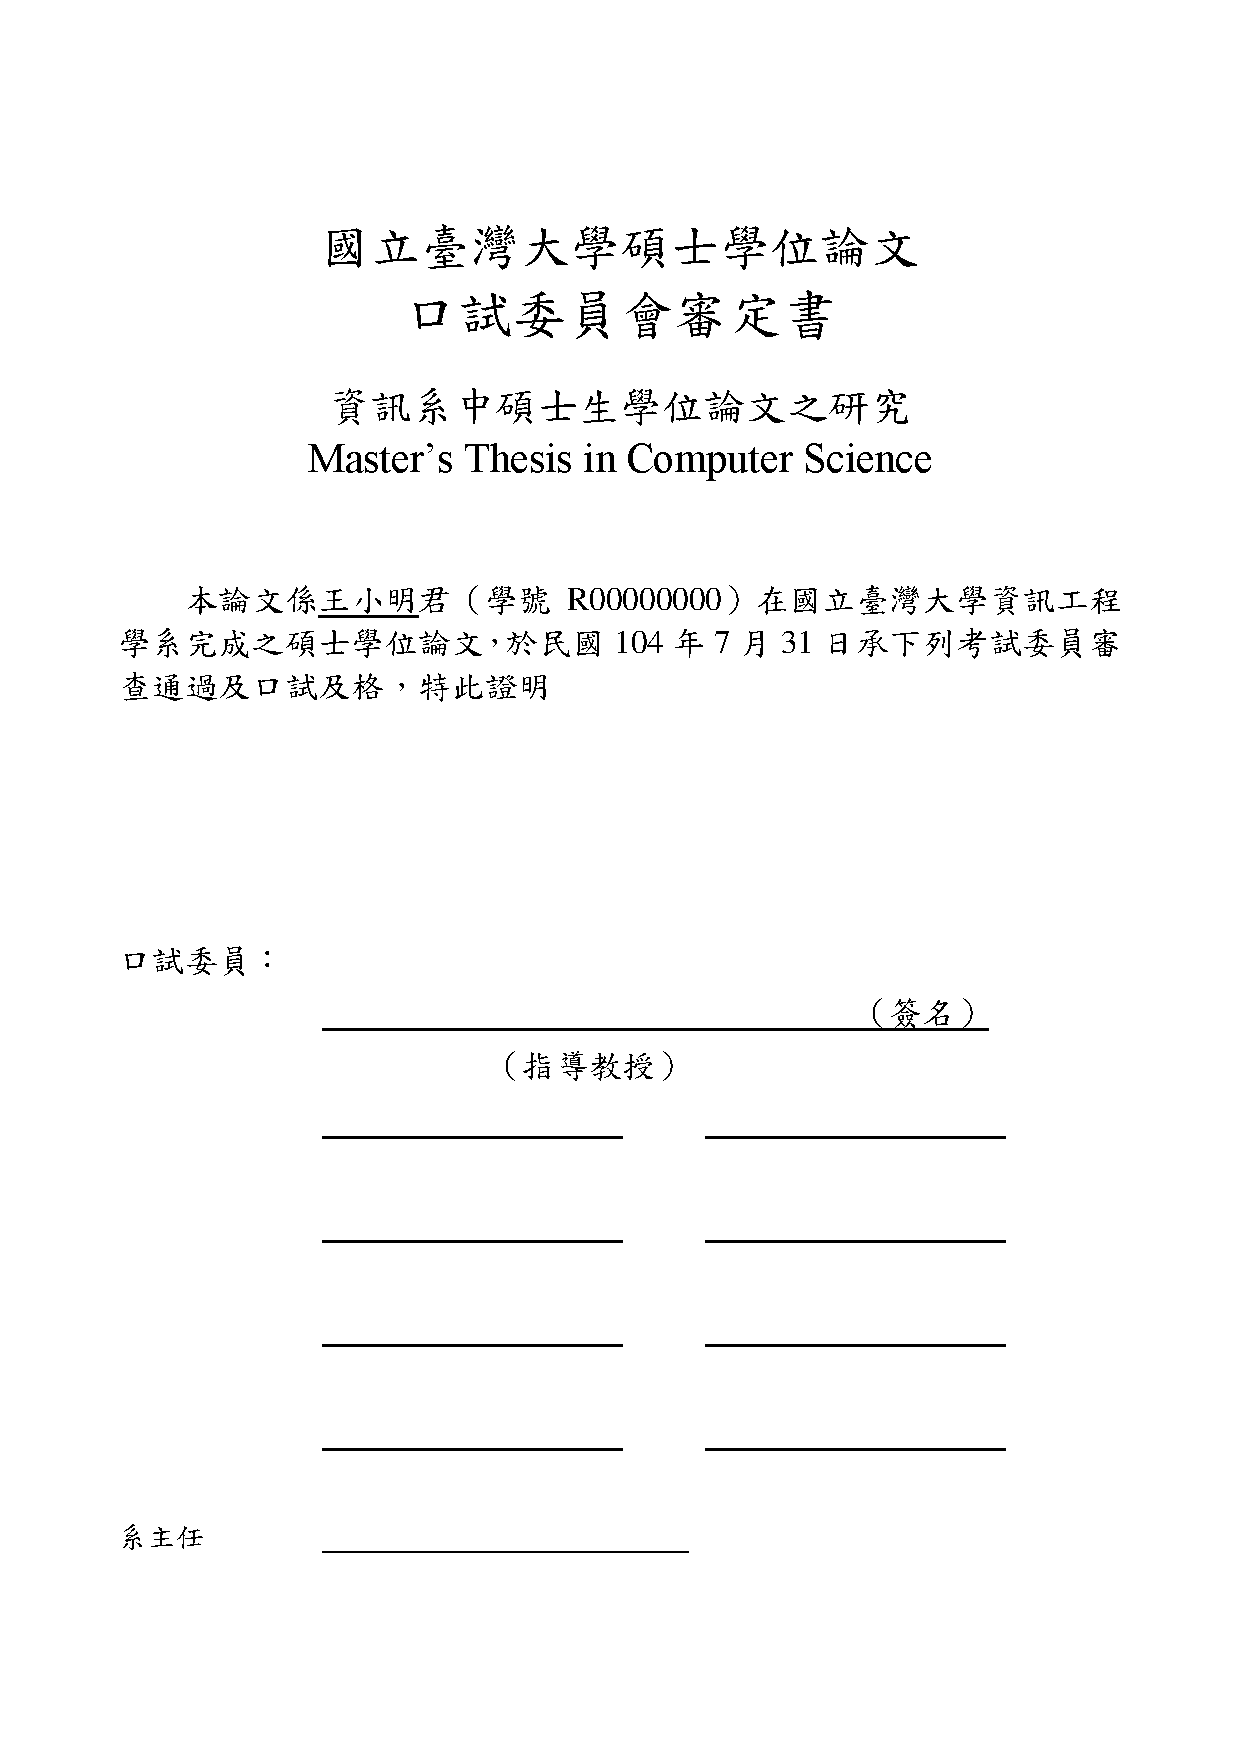
\includepdf[pages={1}]{pdfs/cert.pdf}

\begin{acknowledgementszh}
這是中文行距測試,應該看到一點五倍行距。這是中文行距測試,應該看到一點
五倍行距。這是中文行距測試,應該看到一點五倍行距。這是中文行距測試,應
該看到一點五倍行距。這是中文行距測試,應該看到一點五倍行距。這是中文行
距測試,應該看到一點五倍行距。這是中文行距測試,應該看到一點五倍行距。
這是中文行距測試,應該看到一點五倍行距。這是中文行距測試,應該看到一點
五倍行距。這是中文行距測試,應該看到一點五倍行距。這是中文行距測試,應
該看到一點五倍行距。這是中文行距測試,應該看到一點五倍行距。這是中文行
距測試,應該看到一點五倍行距。這是中文行距測試,應該看到一點五倍行距。

感謝\ldots
\end{acknowledgementszh}

\begin{acknowledgementsen}
This is English line spacing test. You should see double spacing text.
This is English line spacing test. You should see double spacing text.
This is English line spacing test. You should see double spacing text.
This is English line spacing test. You should see double spacing text.
This is English line spacing test. You should see double spacing text.
This is English line spacing test. You should see double spacing text.
This is English line spacing test. You should see double spacing text.
This is English line spacing test. You should see double spacing text.

I'm glad to thank\ldots 
\end{acknowledgementsen}

\begin{abstracten}
The distributed ledger has been widely used in different scenarios after the Bitcoin turns out.
Unlike the Proof of work (PoW) approaches, there’s another mechanism that used to implement on the decentralize database or fault-tolerate system that have great potential to be transplanted to nowadays consortium blockchain systems.
The research focus on the applying of consensus algorithm to financial organizations with the asynchronous network condition, byzantine attackers and permissioned policy in the system.
We designed a novel algorithm that can tolerate at most no more than one third faulty nodes within the system, which is similar to the previous works but will have better performance base on our mathematical analysis and results of experiences.\\

\noindent
Keywords: NCCU, Blockchain, Consensus Algorithm, Distributed System. 
\end{abstracten}


% Table of Content
\clearpages
\tableofcontents
% List of Figures
\clearpages
\listoffigures
% List of Tables
\clearpages
\listoftables

\mainmatter

% Your thesis goes here
\chapter{Introduction}
\label{c:intro}


\chapter{System Model}
\label{c:sysmodel}
% async. network assumption
We assume the network condition of our system is under the asynchronous assumption, 
which means there exist a bounded network delay $d_a$ that won't be known before the algorithm start to execute. \par

% byzantine failure model

% cryptographic techniques

% adversaries' abilities
%1. can coordinate with the other faulty nodes in the system
%2. can delay the message but not indefinitely
%3. can send any kind of message they want but all normal node would only accept the one in the predefined format
%3. can't subvert the cryptographic techniques

\section{Notations}
see the table~\ref{2-1}
\begin{table}[htbp]
\caption{Table of Notation}
\begin{center}% used the environment to augment the vertical space
% between the caption and the table
\label{2-1}
\begin{adjustbox}{max width=1.1\textwidth}
\begin{tabular}{r c p{0cm} }
\toprule

$N_{i}$ & Node in the system with index $i$.&\\
${F}_{j}$ & Faulty Node in the system with index $j$.&\\
${B}_{b}$ & Block with index $b$.&\\
${H}_{h}$ & Height with index $h$.&\\
${R}_{r}$ & Round with index $r$.&\\
$n$ & Number of nodes in the system.&\\
$f$ & Number of faulty nodes in the system.&\\
$d_{a}$ & Asynchronous network delay.&\\
$d_{s}$ & Synchronous network delay.&\\
$i$ & Index value for nodes in the system.&\\
$j$ & Index value for faulty nodes in the system.&\\
$b$ & Index value for blocks in the system.&\\
$h$ & Index value for heights in the system.&\\
$r$ & Index value for rounds in the system.&\\
$NewBlockProposal(H_h,R_r,B_b)_{i}$ & NewBlockProposal signed by node $i$.&\\
$VotingInstruction(H_h,R_r,B_b)_{i}$ & Message signed by node $i$.&\\
$MsigProposal(H_h,R_r,B_b)_{i}$ & VotingInstruction Message signed by node $i$ .&\\
$Vote(H_h,R_r,B_b)_{i}$ & Vote Message signed by node $i$.&\\
$Commit(H_h,R_r,B_b)_{i}$ & Commit Message signed by node $i$.&\\

\bottomrule
\end{tabular}
\end{adjustbox}
\end{center}
\end{table}

\section{Assumptions}

\chapter{Algorithms}
\label{c:algo}

\section{Normal Operation}
\section{Round Change}
\section{Asynchronous Network Condition}
\section{Different Entry Time}
\chapter{Analysis}
\label{c:analysis}
dd

\chapter{Implementation}
\label{c:implement}

\chapter{Experiments}
\label{c:experiment}

There is a tree in Figure~\ref{i:tree}.
This is English line spacing test. You should see double spacing text.
This is English line spacing test. You should see double spacing text.
This is English line spacing test. You should see double spacing text.

%i:tree
\input{figures/tree}

There is a barchart in Figure~\ref{i:barchart}.
This is English line spacing test. You should see double spacing text.
This is English line spacing test. You should see double spacing text.
This is English line spacing test. You should see double spacing text.

%i:barchart
\input{figures/barchart}

%Our method outperforms state-of-art systems as shown in Table~\ref{t:results}.
This is English line spacing test. You should see double spacing text.
This is English line spacing test. You should see double spacing text.
This is English line spacing test. You should see double spacing text.

%t:results
%\input{tables/results}

\chapter{Related Work}
\label{c:related}

%\section{First}
%\label{s:related1}

This is English line spacing test. You should see double spacing text.
This is English line spacing test. You should see double spacing text.
This is English line spacing test. You should see double spacing text.
This is English line spacing test. You should see double spacing text.
This is English line spacing test. You should see double spacing text.
This is English line spacing test. You should see double spacing text.
This is English line spacing test. You should see double spacing text.
This is English line spacing test. You should see double spacing text.
This is English line spacing test. You should see double spacing text.
This is English line spacing test. You should see double spacing text.
This is English line spacing test. You should see double spacing text.
This is English line spacing test. You should see double spacing text.
This is English line spacing test. You should see double spacing text.
This is English line spacing test. You should see double spacing text.
This is English line spacing test. You should see double spacing text.
This is English line spacing test. You should see double spacing text.
This is English line spacing test. You should see double spacing text.
This is English line spacing test. You should see double spacing text.
This is English line spacing test. You should see double spacing text.
This is English line spacing test. You should see double spacing text.
This is English line spacing test. You should see double spacing text.
This is English line spacing test. You should see double spacing text.
This is English line spacing test. You should see double spacing text.
This is English line spacing test. You should see double spacing text.

%\section{Second}

This is English line spacing test. You should see double spacing text.
This is English line spacing test. You should see double spacing text.
This is English line spacing test. You should see double spacing text.
This is English line spacing test. You should see double spacing text.
This is English line spacing test. You should see double spacing text.
This is English line spacing test. You should see double spacing text.
This is English line spacing test. You should see double spacing text.
This is English line spacing test. You should see double spacing text.
This is English line spacing test. You should see double spacing text.
This is English line spacing test. You should see double spacing text.
This is English line spacing test. You should see double spacing text.
This is English line spacing test. You should see double spacing text.
This is English line spacing test. You should see double spacing text.
This is English line spacing test. You should see double spacing text.
This is English line spacing test. You should see double spacing text.
As discussed in Section and Chapter~\ref{c:related}.

\chapter{Conclusions}
\label{c:conclusion}


\@startappendix

\chapter{Datasets}
\label{c:dataset}


\backmatter

\clearpages
\phantomsection
\addcontentsline{toc}{chapter}{\bibname}
\bibliographystyle{apa}

% Your bibliography goes here
\bibliography{thesis}

\end{document}
